% Blabla Matériel et Méthodes

In this part, will be detailed all the hardware, software and methods used to carry out simulations. 

\section{Hardware and Software}

    As this internship is 100\% digital, a good comuter is required. A personal computer (MacBook Air M1) as well as a computer provided by the laboratory (under Ubuntu) will be the main equipment for this internship. \medskip

    The main softwares are the following ones:

    \begin{enumerate}[\hspace{3em}$\bullet$]
        \item \textbf{Visual Studio Code (VS Code)}: a source-code editor developed by Microsoft.
        \item \textbf{Large-scale Atomic/Molecular Massively Parallel Simulator (LAMMPS)}: a molecular dynamics programm (coded in \verb|C++|) from \href{http://www.sandia.gov}{Sandia National Laboratories}.
        \item \textbf{Perseus Gricad}: high performance computing and storage platforms.  
        \item \textbf{Ovito}: a visualization and analysis software for output data generated in molecular dynamics. 
    \end{enumerate}

    \subsection{LAMMPS}

        LAMMPS is an open-source molecular dynamic code with a focus on materials modeling. It provides potentials for solid-state materials (metals and semiconductors). It can be used to model atoms or, more generically, as a parallel particle simulator at the atomic, meso, or continuum scale. \medskip

        LAMMPS does not have any graphic interface which makes the handholding not that easy. The input code is written is \verb|.txt| files thats are compilled through a \verb|Makefile| called with a \verb|bash| command : \verb|lmp_serial -in input.file.txt|.
        
        LAMMPS provides a \verb|log.lammps| file as output. All the behaviour of the script (output values, warnings, errors \dots) is written in this file. However, with specific commands, this software can provide other outfile such as a \verb|dump.test| file, which will be useful to have a visualization of the material behaviour. \medskip

        Here is a quick recap : 

        \begin{center}
            \captionsetup{type=figure}
            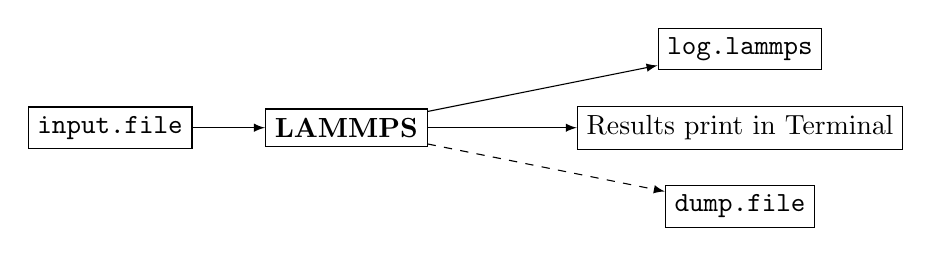
\begin{tikzpicture}
                \node[draw](I) at (0,0) {\verb|input.file|};
                \node[draw](L) at (3,0) {\textbf{LAMMPS}};
                \node[draw](LOG) at (8,1) {\verb|log.lammps|};
                \node[draw](RES) at (8,0) {Results print in Terminal};
                \node[draw](D) at (8,-1) {\verb|dump.file|};
                \draw[->,>=latex] (I) -- (L);
                \draw[->,>=latex] (L) -- (LOG);
                \draw[->,>=latex] (L) -- (RES);
                \draw[->,>=latex,dashed] (L) -- (D);
            \end{tikzpicture}
            \captionof{figure}{LAMMPS operation}
        \end{center}
        